%%%%%%%%%%%%%%%%%%%%%%%%%%%%%%%%%%%%%%%%%%%%%%%%%%%%%%%%%%%%%%%%%%%%%%%%%%%%%
%%%
%%% File: thesis.tex, version 1.9, May 2016
%%%
%%% =============================================
%%% This file contains a template that can be used with the package
%%% cs.sty and LaTeX2e to produce a thesis that meets the requirements
%%% of the Computer Science Department from the Technical University of Cluj-Napoca
%%%%%%%%%%%%%%%%%%%%%%%%%%%%%%%%%%%%%%%%%%%%%%%%%%%%%%%%%%%%%%%%%%%%%%%%%%%%%

\documentclass[12pt,a4paper,twoside]{report}         
\usepackage{cs}              
\usepackage{times}
\usepackage{graphicx}
\usepackage{tikz}
\usepackage{latexsym}
\usepackage{amsmath,amsbsy}
\usepackage{amssymb}
\usepackage[matrix,arrow]{xy}
\usepackage[T1]{fontenc}
\usepackage{ae,aecompl}
\usepackage{romanian} %definitii pentru diacritice; 
\usepackage{amstext}
\usepackage{graphics}
\usepackage[T1]{fontenc}
\usepackage{ae,aecompl}
\usepackage{algorithm}
%\usepackage{algorithmic}
\usepackage{color}
\usepackage{color}
\usepackage{makecell}
\usepackage{eurosym}

\usepackage{pifont}% http://ctan.org/pkg/pifont

% \mastersthesis
\diplomathesis
% \leftchapter
\centerchapter
% \rightchapter
\singlespace
% \oneandhalfspace
% \doublespace

\renewcommand{\thesisauthor}{Diana BEJAN}    %% Your name.
\renewcommand{\thesismonth}{Iulie}     %% Your month of graduation.
\renewcommand{\thesisyear}{2019}      %% Your year of graduation.
\renewcommand{\thesistitle}{SISTEM DE STOCARE A FISIERELOR} % Title
\renewcommand{\thesissupervisor}{ Senior Lector Eng. Cosmina IVAN}
\newcommand{\department}{FACULTATEA DE AUTOMATIC'A 'SI CALCULATOARE\\
DEPARTAMENTUL CALCULATOARE}
\newcommand{\thesis}{LUCRARE DE LICEN'T'A}
\newcommand{\uline}[1]{\rule[0pt]{#1}{0.4pt}}
%\renewcommand{\thesisdedication}{P'arin'tilor mei}
\newcommand{\utcnlogo}{
\includegraphics[width=15cm]{img/utcn.jpg}}
\newcommand{\greencheck}{\color{green}  \ding{51}}
\newcommand{\orangepm}{\color{orange} \textbf{$\pm$}}

\newcommand{\redxmark}{\color{red} \ding{55}}

\begin{document}
%\frontmatter
%\pagestyle{headings}

\newenvironment{definition}[1][Defini'tie.]{\begin{trivlist}
\item[\hskip \labelsep {\bfseries #1}]}{\end{trivlist}}



%\thesistitle                    %% Generate the title page.
%\authordeclarationpage                %% Generate the declaration page.

\pagenumbering{arabic}
\setcounter{page}{4}



\begin{center}
%\includegraphics[width=15cm]{img/tucn.jpg}  
\utcnlogo

{\bf \department}

\vspace{4cm}

{\bf \thesistitle} %LICENSE THESIS TITLE}

\vspace{1.5cm}

\thesis

\vspace{6cm}

Absolvent: {\bf \thesisauthor} 

Conduc'ator 'stiin'tific: {\bf \thesissupervisor}

\vspace{3cm}
{\bf \thesisyear}
\end{center}

\thispagestyle{empty}
\newpage

\begin{center}
\utcnlogo

{\bf \department}
\end{center}
\vspace{0.5cm}

%\begin{small}
\begin{tabular}{p{7cm}p{8cm}}
 %\hspace{-1cm}& VIZAT,\\
 \hspace{-1cm}DECAN, & DIRECTOR DEPARTAMENT,\\
\hspace{-1cm}{\bf Prof. dr. ing. Liviu MICLEA} & {\bf Prof. dr. ing. Rodica POTOLEA}\\  
\end{tabular}
 
\vspace{2cm}

\begin{center}
Absolvent: {\bf \thesisauthor}

\vspace{1cm}

{\bf \thesistitle}
\end{center}

\vspace{1cm}

\begin{enumerate}
 \item {\bf Enun'tul temei:} Crearea unui sistem de stocare a fisierelor in cloud, acesta fiind disponibil sub forma de  mobile(IOS si Android) si  de aplica'tie web. Aplica'tia realizazeaz'a stocarea fi'sierelor 'in forma criptat'a, pentru a oferi protec'tie sporit'a a datelor, 'si compresat'a pentru utilizarea eficient'a a spa'tiului de stocare al utilizatorului. De asemenea sistemul ofer'a un mecanism de restabilire a datelor printr-un sistem de logare avansat.
\item {\bf TODO Con'tinutul lucr'arii:} {\it (enumerarea p'ar'tilor componente) Exemplu: Pagina de prezentare, aprecierile coordonatorului de lucrare, titlul capitolului 1, titlul capitolului 2, titlul capitolului n, bibliografie, anexe.}
\item {\bf Locul document'arii:} Universitatea Tehnic'a din Cluj-Napoca, Departamentul Calculatoare
\item {\bf Consultan'ti:} Senior Lector Eng. Cosmina Ivan
\item {\bf Data emiterii temei:} 21 ianuarie 2019
\item {\bf Data pred'arii:} 17 iulie 2019
  \end{enumerate}
\vspace{1.2cm}

\hspace{6cm} Absolvent: \uline{6cm} 

\vspace{0.5cm}
\hspace{6cm} Coordonator 'stiin'tific: \uline{5cm} 
%\end{small}

\thispagestyle{empty}


\newpage
$ $
%\begin{center}
%\utcnlogo

%{\bf \department}
%\end{center}

\thispagestyle{empty}
\newpage

\begin{center}
\utcnlogo

{\bf \department}
\end{center}

\vspace{0.5cm}

\begin{center}
{\bf
Declara'tie pe proprie r'aspundere privind\\ 
autenticitatea lucr'arii de licen't'a}
\end{center}
\vspace{1cm}



Subsemnatul(a) \\
\uline{14.8cm}, 
legitimat('a) cu \uline{4cm} seria \uline{3cm} nr. \uline{4cm}\\
CNP \uline{9cm}, autorul lucr'arii \uline{2.8cm}\\
\uline{16cm}\\
\uline{16cm}\\
elaborat'a 'in vederea sus'tinerii examenului de finalizare a studiilor de licen't'a la Facultatea de Automatic'a 'si Calculatoare, Specializarea \uline{7cm} din cadrul Universit'a'tii Tehnice din Cluj-Napoca, sesiunea \uline{4cm} a anului universitar \uline{3cm}, declar pe proprie r'aspundere, c'a aceast'a lucrare este rezultatul propriei activit'a'ti intelectuale, pe baza cercet'arilor mele 'si pe baza informa'tiilor ob'tinute din surse care au fost citate, 'in textul lucr'arii 'si 'in bibliografie.

Declar, c'a aceast'a lucrare nu con'tine por'tiuni plagiate, iar sursele bibliografice au fost folosite cu respectarea legisla'tiei rom\ia ne 'si a conven'tiilor interna'tionale privind drepturile de autor.

Declar, de asemenea, c'a aceast'a lucrare nu a mai fost prezentat'a 'in fa'ta unei alte comisii de examen de licen't'a.

'In cazul constat'arii ulterioare a unor declara'tii false, voi suporta sanc'tiunile administrative, respectiv, \emph{anularea examenului de licen't'a}.

\vspace{1.5cm}

Data \hspace{8cm} Nume, Prenume

\vspace{0.5cm}

\uline{3cm} \hspace{5cm} \uline{5cm}

\vspace{1cm}
\hspace{9.4cm}Semn'atura

\thispagestyle{empty}

\newpage


%\listoftables
%\listoffigures

%\clearpage 
%\newpage

%\begin{comment}
{\color{red}{\bf De citit 'inainte} (aceast'a pagin'a se va elimina din versiunea final'a)}:
\begin{enumerate}
 \item Cele trei pagini anterioare (foaie de cap'at, foaie sumar, declara'tie) se vor lista pe foi separate (nu fa't'a-verso), fiind incluse 'in lucrarea listat'a. 
 Foaia de sumar (a doua) necesit'a semn'atura absolventului, respectiv a coordonatorului.
 Pe declara'tie se trece data c\ia nd se pred'a lucrarea la secretarii de comisie.
 \item Pe foaia de cap'at, se va trece corect titulatura cadrului didactic 'indrum'ator, 'in englez'a (consulta'ti pagina de unde a'ti desc'arcat acest document pentru lista cadrelor didactice cu titulaturile lor).
 \item Documentul curent {\bf nu} a fost creat 'in MS Office. E posibil sa fie mici diferen'te de formatare. 
\item Cuprinsul 'incepe pe pagina nou'a, impar'a (dac'a se face listare fa't'a-verso), prima pagin'a din capitolul Introducere tot a'sa, fiind numerotat'a cu 1. % Pentru actualizarea cuprinsului, click dreapta pe cuprins (zona cuprinsului va apare cu gri), Update field-$>$Update entire table.
\item Vizualiza'ti (recomandabil 'si 'in timpul edit'arii) acest document % după ce activaţi vizualizarea simbolurilor ascunse de formatare (apăsaţi simbolul  din Home/Paragraph).
\item Fiecare capitol 'incepe pe pagin'a nou'a. % datorită simbolului ascuns Section Break (Next Page) care este deja introdus la capitolul precedent. Dacă ştergeţi din greşeală simbolul, se reintroduce (Page Layout -> Breaks).
\item Folosi'ti stilurile predefinite (Headings, Figure, Table, Normal, etc.)
\item Marginile la pagini nu se modific'a.
\item Respecta'ti restul instruc'tiunilor din fiecare capitol.
\end{enumerate}
 
%\end{comment}

\newpage

\tableofcontents
\newpage



\chapter{Introducere - Contextul proiectului}
\pagestyle{headings}
'In epoca contemporan'a se observ'a o tendin't'a continu'a a digitaliz'arii si transform'arii digitale, fapt care aduce un impact enorm atât asupra marilor companii, atât 'si asupra utilizatorilor individuali. Lumea bazat'a pe date va fi permanent'a, mereu 'in urm'arire, mereu 'in stadiu de monitorizare - pentru c'a va fi mereu 'in stadiu de 'inv'a'tare.
IDC \cite{IDCdigitization}  a definit trei loca'tii principale 'in care digitalizarea are loc 'si unde este creat con'tinutul de date: tip nucleu (centre de date tradi'tionale si de tip cloud), tip muchie (infrastructuri de tip sucursal'a), 'si obiectivele finale (PC-uri, telefoane si dispozitive IoT). Sumarizarea tuturor acestor date, 'in momentul 'in care sunt  create, capturate sau replicate, se nume'ste Global Datasphere, 'si aceasta se confrunt'a cu o cre'stere spectaculoas'a. IDC (International Data Corporation) estimeaz'a c'a volumul de date din Global Datasphere va cre'ste de la 33 Zettabytes\footnote{1 Zetta byte echivalent cu $2^{70}$ bytes} 'in 2018 pân'a la 175 Zettabytes in 2025.
'In trecutul recent utilizatorii erau responsabili pentru datele lor, 'insa dependen'ta 'si 'increderea lor 'in servciile cloud, 'in special din  cauza conectivit'a'tii, performan'tei si confortului, continua sa creasc'a ceea ce duce la noi provoc'ari pentru furnizorii de servicii cloud. Mediul afarcerilor urm'are'ste centralizarea managementului datelor, pentru a putea oferi securitate, analiz'a de date, experien't'a utilizator mai bun'a (prin comunicare 'intre dispozitive, IoT, personalizarea profilului). Responsabilitatea pentru managementul datelor utilizatorilor 'si businessurilor duce la o crestere continu'a a centrelor de date ale furnizorilor de servicii Cloud. Ca rezultat importan'ta serviciilor cloud cre'ste considerabil, iar utilizatorii nu doar permit acest lucru si se a'stteapt'a la o crestere cât mai spectaculoas'a.

\section{Context general}


\section{Contextul proiectului}


\section{Contextul proiectului}
\section{Continutul proiectului}
\subsection{Microservicii}

Fiecare tabel introdus 'in lucrare este numerotat astfel: Tabel x.y, unde x reprezint'a num'arul capitolului iar y num'arul tabelului din capitol. 
Se las'a un r\ia nd liber 'intre tabel 'si paragraful anterior, respectiv posterior (table~\ref{table:nonlin}).

\begin{table}[ht]
\caption{Rezultate}
\centering                          % tabel centrat 
\begin{tabular}{|c|c|c|c|}          % 4 coloane centrate 
\hline\hline                        % linie orizontala dubla
Case & Method\#1 & Method\#2 & Method\#3 \\ [0.5ex]   % inserare tabel
%heading
\hline                              % linie orizontal simpla
1 & 50 & 837 & 970 \\               % corpul tabelului 
2 & 47 & 877 & 230 \\
3 & 31 & 25 & 415 \\[1ex]           % [1ex] adds vertical space
\hline                              
\end{tabular}
  % titlul tabelului
\label{table:nonlin}                % \label{table:nonlin} introduce eticheta folosita pentru referirea tabelului in text; referirea in text se va face cu \ref{table:nonlin}
\end{table}

Fiecare figur'a introdus'a 'in text este citat'a (de ex: 'in figura x.y este prezentat'a ...) 'si numerotat'a. 
Numerotarea se face astfel Figura x.y unde x reprezint'a num'arul capitolului iar y num'arul figurii 'in acel capitol. 
E.g.: figure~\ref{fig:imag}.

\begin{figure}[ht]
    \centering
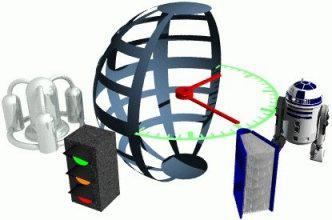
\includegraphics[]{img/test.jpg}
    \caption{Numele figurii}
    \label{fig:imag}
\end{figure}

Fiecare capitol 'incepe pe pagin'a nou'a.

\chapter{Obiectivele Proiectului}

'In acest capitol se prezint'a tema propriu-zis'a (sub forma unei teme de proiectare sau cercetare, formulat'a exact, cu obiective clare - 2-3 pagini 'si eventuale figuri explicative).

Reprezint'a cca. 10\% din lucrare.
\section{Obiective principale}
\section{Obiective generale}
\section{Obiective specifice}


\chapter{Studiu Bibliografic}

Documentarea bibliografic'a are ca obiectiv prezentarea stadiului actual al domeniului sau sub-domeniului 'in care se situeaz'a tema. 
'In redactarea acestui capitol ('in general a 'intregului document) se va 'tine cont de cuno'stin'tele acumulate la disciplinele dedicate din semestrul 2, anul 4 
(Metodologia 'Intocmirii Proiectelor, etc.), precum 'si la celelalte discipline relevante temei abordate.

Acest capitol reprezint'a cca. 15\% din lucrare.

Referin'tele se scriu 'in sec'tiunea Bibliografie. 
Formatul referin'telor trebuie s'a fie de tipul IEEE sau asem'an'ator. 
Introducerea 'si formatarea referin'telor 'in bibliografie, respectiv citarea 'in text, se pot face manual sau folosind instrumentele de lucru men'tionate 'in ultimele paragrafe din acest capitol.




In chapter~\ref{ch:analysis} of~\cite{strunk}, which discusses the value of the honeypots, Spitzner presents the advantages and disadvantages of such systems. 


'In sec'tiunea {\it Bibliografie} sunt exemple de referin'te pentru articol la conferin'te sau seminarii~\cite{BellucciLZ04}, articol 'in jurnal~\cite{AntoniouSBDB07}, 
sau c'ar'ti~\cite{russell1995artificial}. 


Referin'tele spre aplica'tii sau resurse online (pagini de internet) trebuie sa includ'a cel pu'tin o denumire sugestiv'a pe l\ia ng'a link-ul propriu-zis~\cite{webpage}, 
plus alte informa'tii dac'a sunt disponibile (autori, an, etc.). 
Referin'tele care prezint'a doar link spre resursa online se vor plasa 'in subsolul paginii unde sunt referite.
Citarea referin'telor 'in text este obligatorie, vezi exemplul de mai jos ('in func'tie de tema proiectului se poate varia modul de prezentare a metodei/aplica'tiei).

%'In articolul~\cite{AntoniouSBDB07} autorii prezint'a un sistem pentru ...
'In~\cite{AntoniouSBDB07} autorii prezint'a un sistem pentru detec'tia obstacolelor 'in mi'scare folosind stereoviziune 'si estimarea mi'sc'arii proprii. 
Metoda se bazeaz'a pe ...{\it trecere 'in revist'a a algoritmilor, structurilor de date, func'tionalitate, aspecte specifice temei proiectului etc}. Discu'tie {\it avantaje - dezavantaje}.


'In capitolul~\ref{ch:analysis} al~\cite{russell1995artificial} se prezint'a ...  

\section{Microservicii}
\subsection{Arhitectura monolitic'a} 

\subsection{Dezavantajele  arhitecturii monoliitice}

\subsection{Caracteristicile arhitecturii bazate pe microservicii}

\subsection{Avantajele arhitecturii bazate pe microservicii}

\subsection{Provoc'ari} 

\section{Securitatea in sistemele informatice}

\subsection{Amenin'tári}

\subsection{Aspecte ale securitatii systemelor}

\subsection{Criptarea datelor}

\section{Cloud}

\subsection{Beneficii si impedimente}

\subsection{Microservicii in Cloud}

\section{Sisteme similare}
Acest capitol reprezint'a clasificarea si analiza sistemelor similare existente, bazat'a pe etapa de cercetare a proiectului. Sistemele au scop 'si functionalit'a'ti similare cu proiectul propus. Sistemele alese pentru compara'tie sunt:
\begin{itemize}
\item[•] CloudMe
\item[•] Dropbox
\item[•] CrashPlan
\item[•] ICloud
\item[•] Google Drive
\item[•] OneDrive
\item[•] pCloud
\item[•] sync.com
\end{itemize}
Dropbox, Google Drive, ICloud si OneDrive au fost incluse 'in acest studiu deoarece sunt 'in top 10 cele mai populare servicii de cloud 2019 \cite{topcloud}.Acestea reprezint'a un model pentru cum este v'azut un cloud storage modern: simplu de configurat, simplu de utilizat 'si disponibil la un pre't avantajos.
pCloud si sync.com sunt 'in topul sistemelor cu cea mai 'inalt'a recuritate de pe pia't'a. pCloud este categorizat ca un sistem infraudabil 'si nu a avut nici o expunere a datelor utilizatorilor. 'Ins'a aceste sisteme vin si cu pre'turi de 3-4 ori mai mari decât sistemele clasice.
\subsection{Metodologia de analiz'a}
'In ultimul deceniu tot mai mul'ti utilizatori, atât business cât 'si individuali, se baseaz'a pe stocarea fi'sierelor 'in Cloud.  Cele mai importante criterii pe care se bazeaz'a utilizatorii sunt: securitatea, simplitatea de utilizare a sistemului, disponibilitatea si pre'tul de utilizare. Analiza sistemelor individuale de cloud a fost efectuat'a 'in modul urm'ator:

Sunt sumarizate pre'turile de utilizare a sistemului 'si a diferitor op'tiuni. Sunt analizate detaliile capabilit'a'tilor tehnice 'si organiza'tionale ale p'ar'tii client 'si server a sistemului. Informa'tiile colectate sunt bazate pe sec'tiunile
{\it  Terms of Service } 'si {\it Privacy Policy} ale documenta'tiilor oficiale ale sistemelor.
\cite{cloudstoragecomparison}
Rezultatele analizei comparative au ca scop determinarea cerin'telor pricipale ale unui sistem de stocare cloud 'si compara'tia sistemului elaborat cu cele existente.
\subsubsection{Formatul analizei}
'In sec'tiunile ce urmeaz'a se vor analiza urm'atoarele func'tionalit'a'ti:

\begin{table}[H]
\caption{Criterii evaluare}
\begin{tabular}{|c|c|c|c|c|c|c|c|}          
\hline                     
Copy & Backup & Sync & Sharing & \makecell{Client-side \\ Encryption} & \makecell{ Server-side \\ encryption} & Compression & Watermarking  \\ [0.5ex]   
%heading
\hline                              
\end{tabular}
  % titlul tabelului
\label{table:criteriatable}             
\end{table}

Pentru fiecare categorie din tabelul \ref{table:criteriatable} se va acorda un punctaj:
\begin{itemize}
\item[\greencheck\greencheck] este echivalent pentru {\it foarte bine}, toate cerin'tele obligatorii pentru func'tionalitatea respectiv'a au fost 'indeplinite 'si câteva dintre cele op'tionale.
\item[\greencheck] este echivalent pentru {\it bine}, adic'a toate cerin'tele obligatorii pentru func'tionalitatea respectiv'a au fost 'indeplinite.
\item[\orangepm] este simbolul pentru {\it bine cu câteva vulnerabilit'a'ti}, nu toate cerin'tele esen'tiale au fost 'indeplinite.
\item[\redxmark] este echivalent cu {\it slab}, cel pu'tin o cerin't'a obligatorie nu a fost 'indeplinit'a.
\item[\redxmark \redxmark] este echivalentul pentru {\it foarte slab}, adic'a mai multe dintre cerin'tele obligatorii nu sunt indeplinite in func'tionalitatea respectiv'a sau func'tionalitatea lipse'ste.

\end{itemize}
\subsection{CloudMe}
\subsubsection{Punctaj}
\begin{table}[H]
\centering
\caption{Func'tionalit'a'ti CloudMe}
\begin{tabular}{|c|c|c|c|c|c|c|c|}          
\hline               
Copy & Backup & Sync & Sharing & \makecell{Client-side\\ Encryption} & \makecell{Server-side \\ encryption} & Compression & Watermarking \\ [0.5ex]   
%heading
\hline 
Da & Da & Da & Da & Da &  Nu & Nu & Nu    \\                      
\greencheck & \greencheck & \redxmark\redxmark & \orangepm & \greencheck\greencheck & \redxmark\redxmark &  \redxmark\redxmark &  \redxmark\redxmark  \\               
\hline                              
\end{tabular}
  % titlul tabelului
\label{table:cloudmefeaturetable}             
\end{table}
\begin{table}[H]
\centering
\caption{Platforme disponibile 'si pre't}
\begin{tabular}{|c|c|c|c|}          
\hline                      
 Web Client & Desktop client & Mobile Client & 500GB Plan Price\\ [0.5ex]   
%heading
\hline                            
Da & Da & Da & 30\euro\\               
\hline                              
\end{tabular}
  % titlul tabelului
\label{table:cloudmesystemtable}             
\end{table}
\subsubsection{Analiz'a}
CloudMe \footnote{https://www.cloudme.com/} este un sistem de cloud standard, care vine cu un serviciu de sincronizare 'si backup a fi'sierelor, dup'a o analiz'a detaliata ne putem da seama c'a acest sistem a fost inspirat din arhicunoscutul Dropbox care este analizat 'in sec'tiunea \ref{dropbox}.

Un fapt bun despre CloudMe este c'a acesta pune la dispozi'tia utilizatorului un spa'tiu de stocare gratuit de 3GB, iar pentru volume de date mai mari ofer'a op'tiuni la pre'tul mediu al pie'tei. Serviciul ofer'a func'tionalit'a'tile de baz'a, 'ins'a nimic desebit 'in materie de securitate. 

Interfa'ta web a CloudMe este foarte simpl'a si clar'a, este evident cum sa 'incarci un fisier sau cum sa 'il schimbi 'in alt folder.
\begin{figure}[H]
\begin{center}
\advance\leftskip-3cm
\advance\rightskip-3cm
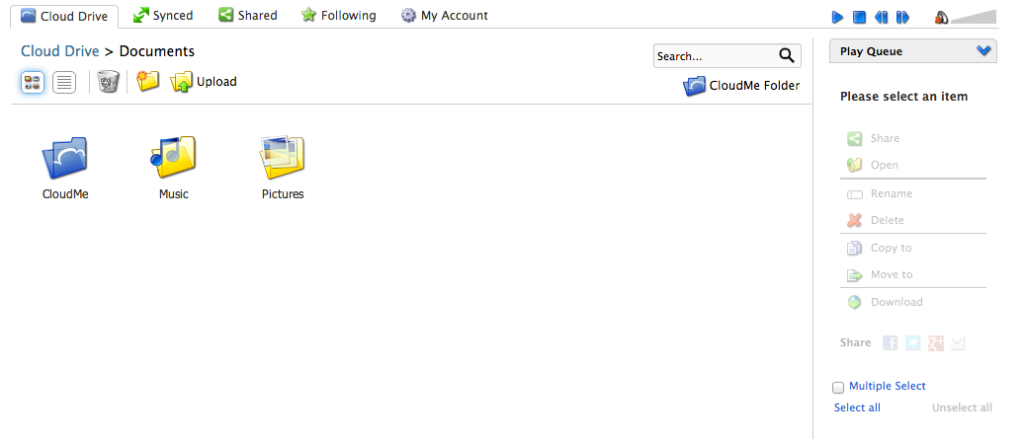
\includegraphics[keepaspectratio=true,scale=0.4]{img/Web-interface_CloudME.png}
\caption{}
\label{web_cloudMe}
\end{center}
\end{figure}

CloudMe ofer'a sincronizarea aplica'tiilor pentru Windows, Mac, Linux, iOS 'si Android. Pentru ca sincronizarea sa poata avea loc utilizatorul prime'ste un a'sa numit "director albastru" ofer'a utilizatorului singronizare 'in timp real. De asemenea CloudMe ofer'a op'tiunea de a alege timpul la care se va 'intâmpla sincronizarea.
Pentru a distribui fi'siere sunt disponibile mai multe op'tiuni, 'incepând cu distribuire clasic'a, care permite utilizatorului s'a ofere acces la fi'sierele lui prin distribuirea unui link, 'si ajungând la metode mult mai colaborative care permit altor utilizatori, c'arora li se ofer'a access, s'a modifice fi'sierele din cloudul altui utilizator sau s'a 'incarce fi'siere noi.

\begin{figure}[H]
\begin{center}
\advance\leftskip-3cm
\advance\rightskip-3cm
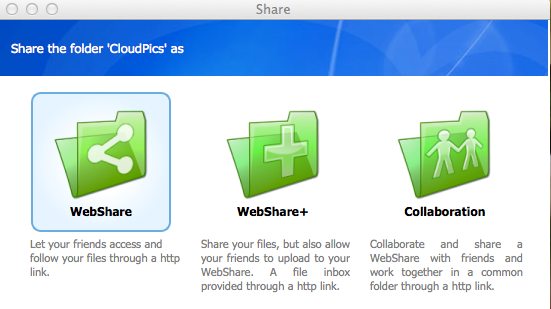
\includegraphics[keepaspectratio=true,scale=0.4]{img/Share-options_CloudME.png}
\caption{}
\label{web_cloudMe}
\end{center}
\end{figure}

CloudMe arhiveaz'a  versiunile precedente ale fi'sierelor  prin func'tionalitatea co'sului de gunoi, care p'astreaz'a pentru 60 de zile toate fi'sierele care au fost 'sterse.

'In privin'ta securit'a'tii ClodMe nu este o op'tiune prea bun'a deoarece nu ofer'a criptarea datelor, acestea fiind vulnerabile pentru atacuri. Este posibil s'a 'incarci 'si s'a descarci fi'siere criptate, 'ins'a criptarea 'si decriptarea acestora ram'ane la latitudinea utilizatorului.

\subsubsection{Concluzii}
CloudMe este o aplica'tie foarte u'sor de utilizat 'si are o interfa't'a foarte intuitiv'a. Acesta dispune de func'tionalit'a'tile de baz'a ale unui sistem de stocare 'in cloud, 'ins'a nu este potrivit pentru stocarea fisierelor cu con'tinut de date senzitiv din cauza lipsei cript'arii, de asemnea atunci c'and fi'sierele sunt distribuite dup'a un link este foarte greu s'a determini cine a f'acut public un fi'sier cu caracter privat deoarece link-ul de acces poate fi u'sor furat.

Un alt defect al acestui sistem este func'tionalitatea de {\it Sync}, motivul pentru care i-am oferit punctaj minim este c'a 'in ultimul an a avut multiple vulnerabilit'a'ti, conform {\it CVE-2018-6892} \footnote{https://nvd.nist.gov/vuln/detail/CVE-2018-6892} atacatorii se puteau conecta la clientul de  "CloudMe Sync" prin portul 8888 'si trimiterea unor date mali'tioase puteau cauza "buffer overflow", acest lucru le oferea control asupra execu'tiei 'si posibilitatea de a executa cod mali'tios.

\subsection{Dropbox} \label{dropbox}
\subsubsection{Punctaj}
\begin{table}[H]
\centering
\caption{Func'tionalit'a'ti Dropbox}
\begin{tabular}{|c|c|c|c|c|c|c|c|}          
\hline               
Copy & Backup & Sync & Sharing & \makecell{Client-side\\ Encryption} & \makecell{Server-side \\ encryption} & Compression & Watermarking \\ [0.5ex]   
%heading
\hline 
Da & Da & Da & Da & Da &  Da  & Nu & Nu    \\                      
\greencheck & \greencheck & \redxmark\redxmark & \orangepm & \greencheck\greencheck & \greencheck\greencheck &  \redxmark\redxmark &  \redxmark\redxmark  \\               
\hline                              
\end{tabular}
  % titlul tabelului
\label{table:dropboxfeaturetable}             
\end{table}
\begin{table}[H]
\centering
\caption{Platforme disponibile 'si pre't}
\begin{tabular}{|c|c|c|c|}          
\hline                      
 Web Client & Desktop client & Mobile Client & 500GB Plan Price\\ [0.5ex]   
%heading
\hline                            
Da & Da & Da & 18\euro \\               
\hline                              
\end{tabular}
  % titlul tabelului
\label{table:dropboxsystemtable}             
\end{table}
\subsubsection{Analiz'a}
Vulneralititati arbitrary bypass.

\subsection{CrashPlan}
\subsubsection{Punctaj}
\begin{table}[H]
\centering
\caption{Func'tionalit'a'ti}
\begin{tabular}{|c|c|c|c|c|c|c|c|}          
\hline               
Copy & Backup & Sync & Sharing & \makecell{Client-side\\ Encryption} & \makecell{Server-side \\ encryption} & Compression & Watermarking \\ [0.5ex]   
%heading
\hline 
Da & Da & Da & Nu & Da &  Da  & Nu & Nu    \\                      
\greencheck & \greencheck & \redxmark\redxmark & \redxmark\redxmark & \greencheck\greencheck & \orangepm &  \redxmark\redxmark &  \redxmark\redxmark  \\               
\hline                              
\end{tabular}
  % titlul tabelului
\label{table:crashplanfeaturetable}             
\end{table}
\begin{table}[H]
\centering
\caption{Sisteme de operare}
\begin{tabular}{|c|c|c|c|}          
\hline                      
 Web Client & Desktop client & Mobile Client & 500GB Plan Price\\ [0.5ex]   
%heading
\hline                            
Da & Da & No & 10\euro \\               
\hline                              
\end{tabular}
  % titlul tabelului
\label{table:crashplansystemtable}             
\end{table}
\subsubsection{Analiz'a}
Remote Code Execution is possible in Code42 CrashPlan 5.4.x via the org.apache.commons.ssl.rmi.DateRMI Java class, because (upon instantiation) it creates an RMI server that listens on a TCP port and deserializes objects sent by TCP clients.	
\subsection{ICloud}

\subsubsection{Punctaj}
\begin{table}[H]
\centering
\caption{Func'tionalit'a'ti}
\begin{tabular}{|c|c|c|c|c|c|c|c|}          
\hline               
Copy & Backup & Sync & Sharing & \makecell{Client-side\\ Encryption} & \makecell{Server-side \\ encryption} & Compression & Watermarking \\ [0.5ex]   
%heading
\hline 
Da & Da & Da & Da & Da & Nu & Nu & Nu    \\                      
\greencheck & \greencheck & \greencheck\greencheck & \greencheck & \greencheck\greencheck & \redxmark\redxmark &  \redxmark\redxmark &  \redxmark\redxmark  \\               
\hline                              
\end{tabular}
  % titlul tabelului
\label{table:icloudfeaturetable}             
\end{table}
\begin{table}[H]
\centering
\caption{Sisteme de operare}
\begin{tabular}{|c|c|c|c|}          
\hline                      
 Web Client & Desktop client & Mobile Client & 500GB Plan Price\\ [0.5ex]   
%heading
\hline                            
Da & Da & Da & 10\euro \\               
\hline                              
\end{tabular}
  % titlul tabelului
\label{table:icloudsystemtable}             
\end{table}
\subsubsection{Analiz'a}
https://www.cvedetails.com/cve/CVE-2018-20506/ 

https://www.cvedetails.com/cve/CVE-2018-4464/

https://www.cvedetails.com/cve/CVE-2018-20506/

https://appleinsider.com/articles/18/09/06/spyware-maker-mspy-exposes-icloud-info-as-part-of-massive-data-breach
\subsection{Google Drive}
\subsubsection{Punctaj}
\begin{table}[H]
\centering
\caption{Func'tionalit'a'ti}
\begin{tabular}{|c|c|c|c|c|c|c|c|}          
\hline               
Copy & Backup & Sync & Sharing & \makecell{Client-side\\ Encryption} & \makecell{Server-side \\ encryption} & Compression & Watermarking \\ [0.5ex]   
%heading
\hline 
Da & Da & Da & Da & Da & Nu & Da & Nu    \\                      
\greencheck & \greencheck\greencheck & \greencheck & \greencheck & \greencheck\greencheck & \redxmark\redxmark &  \orangepm &  \redxmark\redxmark  \\               
\hline                              
\end{tabular}
  % titlul tabelului
\label{table:googledrivefeaturetable}             
\end{table}
\begin{table}[H]
\centering
\caption{Sisteme de operare}
\begin{tabular}{|c|c|c|c|}          
\hline                      
 Web Client & Desktop client & Mobile Client & 500GB Plan Price\\ [0.5ex]   
%heading
\hline                            
Da & Da & Da & 15\euro \\               
\hline                              
\end{tabular}
  % titlul tabelului
\label{table:googledrivesystemtable}             
\end{table}
\subsubsection{Analiz'a}
https://www.cvedetails.com/cve/CVE-2013-0300/
\subsection{OneDrive}
\subsubsection{Punctaj}
\begin{table}[H]
\centering
\caption{Func'tionalit'a'ti}
\begin{tabular}{|c|c|c|c|c|c|c|c|}          
\hline               
Copy & Backup & Sync & Sharing & \makecell{Client-side\\ Encryption} & \makecell{Server-side \\ encryption} & Compression & Watermarking \\ [0.5ex]   
%heading
\hline 
Da & Da & Da & Da & Nu & Nu & Nu & Nu    \\                      
\greencheck & \greencheck\greencheck & \greencheck & \greencheck & \redxmark\redxmark & \redxmark\redxmark &  \redxmark\redxmark &  \redxmark\redxmark  \\               
\hline                              
\end{tabular}
  % titlul tabelului
\label{table:onedrivefeaturetable}             
\end{table}
\begin{table}[H]
\centering
\caption{Sisteme de operare}
\begin{tabular}{|c|c|c|c|}          
\hline                      
 Web Client & Desktop client & Mobile Client & 500GB Plan Price\\ [0.5ex]   
%heading
\hline                            
Da & Da & Da & 15\euro \\               
\hline                              
\end{tabular}
  % titlul tabelului
\label{table:onedrivesystemtable}             
\end{table}
\subsubsection{Analiz'a}
https://www.cvedetails.com/cve/CVE-2018-0593/

\subsection{pCloud}
\subsubsection{Punctaj}
\begin{table}[H]
\centering
\caption{Func'tionalit'a'ti}
\begin{tabular}{|c|c|c|c|c|c|c|c|}          
\hline               
Copy & Backup & Sync & Sharing & \makecell{Client-side\\ Encryption} & \makecell{Server-side \\ encryption} & Compression & Watermarking \\ [0.5ex]   
%heading
\hline 
Da & Nu & Da & Da & Da & Da & Nu & Nu    \\                      
\greencheck & \redxmark\redxmark & \greencheck & \greencheck & \greencheck\greencheck & \greencheck\greencheck &  \redxmark\redxmark &  \redxmark\redxmark  \\               
\hline                              
\end{tabular}
  % titlul tabelului
\label{table:pcloudfeaturetable}             
\end{table}
\begin{table}[H]
\centering
\caption{Sisteme de operare}
\begin{tabular}{|c|c|c|c|}          
\hline                      
 Web Client & Desktop client & Mobile Client & 500GB Plan Price\\ [0.5ex]   
%heading
\hline                            
Da & Da & Da & 15\euro \\               
\hline                              
\end{tabular}
  % titlul tabelului
\label{table:pcloudsystemtable}             
\end{table}
\subsubsection{Analiz'a}

\subsection{sync.com}
\subsubsection{Punctaj}
\begin{table}[H]
\centering
\caption{Func'tionalit'a'ti}
\begin{tabular}{|c|c|c|c|c|c|c|c|}          
\hline               
Copy & Backup & Sync & Sharing & \makecell{Client-side\\ Encryption} & \makecell{Server-side \\ encryption} & Compression & Watermarking \\ [0.5ex]   
%heading
\hline 
Da & Da & Da & Da & Da & Da & Nu & Nu    \\                      
\greencheck & \greencheck\greencheck & \greencheck & \greencheck & \greencheck\greencheck & \greencheck\greencheck &  \redxmark\redxmark &  \redxmark\redxmark  \\               
\hline                              
\end{tabular}
  % titlul tabelului
\label{table:syncfeaturetable}             
\end{table}
\begin{table}[H]
\centering
\caption{Sisteme de operare}
\begin{tabular}{|c|c|c|c|}          
\hline                      
 Web Client & Desktop client & Mobile Client & 500GB Plan Price\\ [0.5ex]   
%heading
\hline                            
Da & Da & Da & 15\euro \\               
\hline                              
\end{tabular}
  % titlul tabelului
\label{table:syncsystemtable}             
\end{table}
\subsubsection{Analiz'a}

\subsection{Concluzii 'si plasarea sistemului}


\chapter{Analiz'a 'si Fundamentare Teoretic'a}
\label{ch:analysis}

'Impreun'a cu capitolul urm'ator trebuie s'a reprezinte aproximativ 60\% din total.

Scopul acestui capitol este de a explica principiile func'tionale ale aplica'tiei implementate. 
Aici se va descrie solu'tia propus'a dintr-un punct de vedere teoretic - explica'ti 'si demonstra'ti propriet'a'tile 'si valoarea teoretic'a:
\begin{itemize}
 \item algoritm utilizat sau propus
\item protocoale utilizate
\item modele abstracte
\item explica'tii/argument'ari logice ale solu'tiei alese
\item structura logic'a 'si func'tional'a a aplica'tiei.
\end{itemize}

{\color{red}
NU SE FAC referiri la implementarea propriu-zis'a. 

NU SE PUN descrieri de tehnologii preluate cu copy-paste din alte surse sau lucruri care nu 'tin strict de proiectul propriu-zis (materiale de umplutur'a).
}


\section{Cerin'te}
\subsection{Cerin'te func'tionale}
\subsection{Cerin'te non-func'tionale}
\section{Cazuri de utilizare}
\subsection{Actori}
\subsection{Modele de cazuri de utilizare}
\section{Arhitectura canceptual'a a sistemului}

\section{Tehnologii}
\subsection{Golang}
\subsection{gRPC}
\subsection{VueJS}
\subsection{Java Android}
\subsection{MongoDB}
\subsection{Couchbase}
\subsection{Redis}
\subsection{HTML, CSS, Bootstrap}
\subsection{JSON Web Token(JWT)}
\subsection{Docker 'si Kubernetes}
\subsection{Google Cloud}
\subsection{Google Pub/Sub}
\subsection{Git}


\chapter{Proiectare de Detaliu 'si Implementare}

'Impreun'a cu capitolul precedent reprezint'a aproximativ 60\% din total.

Scopul acestui capitol este de a documenta aplica'tia dezvoltat'a 'in a'sa fel 'inc\ia t dezvoltarea 'si 'intre'tinerea ulterioar'a s'a fie posibile. 
Cititorul trebuie s'a identifice func'tiile principale ale aplica'tiei din ceea ce este scris aici.
Capitolul ar trebui sa con'tin'a (nu se rezum'a neap'arat la):
\begin{itemize}
 \item schema general'a a aplica'tiei
\item descrierea fiec'arei componente implementate, la nivel de modul
\item diagrame de clase, clase importante 'si metode ale claselor importante.
\end{itemize}
\section{Arhitectura serverului}
\subsection{Descriere general'a}
\subsection{Orchestrarea microserviciilor}
\subsection{Comunicarea 'intre microservicii}
\subsection{Microserviciul de autentificare}
\subsection{Microserviciul antivirus}
\subsection{Microserviciul de c'autare}
\subsection{Microserviciul de criptare}
\subsection{Microserviciul de steganografie}
\subsection{Microserviciul de compresie}
\subsection{Microserviciul de autorizare}
\subsection{Microserviciul de evenimente}
\subsection{Microserviciul de fisiere}
\subsection{Microserviciul de logare}

\subsection{Aplica'tiile steganografiei}
\subsection{Securitate}

\section{Arhitectura aplicatiei web}
\subsection{Descriere general'a}
\subsection{Descrierea componentelor}

\section{Arhitectura aplicatiei mobile}
\subsection{Descriere general'a}
\subsection{Descrierea componentelor}

\chapter{Testare 'si Validare}

\section{Testare automat'a}

\section{Testare manual'a}

Aproximativ 5\% din total

\chapter{Manual de Instalare 'si Utilizare}

'In sec'tiunea de Instalare trebuie s'a detalia'ti resursele software 'si hardware necesare pentru instalarea 'si rularea aplica'tiei, precum 'si o descriere pas cu pas a procesului de instalare. 
Instalarea aplica'tiei trebuie s'a fie posibil'a pe baza a ceea ce se scrie aici.

'In acest capitol trebuie s'a descrie'ti cum se utilizeaz'a aplica'tia din punct de vedere al utilizatorului, f'ar'a a men'tiona aspecte tehnice interne.
Folosi'ti capturi ale ecranului 'si explica'tii pas cu pas ale interac'tiunii. 
Folosind acest manual, o persoan'a ar trebui s'a poat'a utiliza produsul vostru.

\section{Cerin'te preliminare}
\section{Instalare si configurare}

\chapter{Concluzii}

Cca. 5\% din total.
Capitolul ar trebui sa con'tin'a (nu se rezum'a neap'arat la):
\begin{itemize}
 \item un rezumat al contribu'tiilor voastre
\item analiz'a critic'a a rezultatelor ob'tinute
\item descriere a posibilelor dezvolt'ari 'si 'imbun'at'a'tiri ulterioare
\end{itemize}


\section{Contribu'tii 'si rezultate ob'tinute}
\section{Dezvolt'ari ulterioare}


%\addcontentsline {toc}{chapter}{Bibliography} 
\bibliographystyle{IEEEtran} 
\bibliography{thesis}%same file name as for .bib

\definecolor{darkbrown}{rgb}{0.59, 0.29, 0.0}
\definecolor{celestialblue}{rgb}{0.29, 0.59, 0.82}
\definecolor{deepchampagne}{rgb}{0.98, 0.84, 0.65}
\definecolor{munsell}{rgb}{0.0, 0.66, 0.47}

\appendix
\chapter{Sec'tiuni relevante din cod}\label{sectiuni_cod}

\subsubsection{Exemplu de fi'sier \textit{protobuf}}
\begin{tcolorbox}\label{proto_definition}
\scriptsize{
\begin{Verbatim}[commandchars=\\\{\}]

\textcolor{blue}{syntax} = \textcolor{darkbrown}{"proto3"};

\textcolor{blue}{package} \textcolor{darkbrown}{compression_service};
\textcolor{blue}{option} go_package=\textcolor{darkbrown}{"pb"};

\textcolor{blue}{import} \textcolor{darkbrown}{"google/api/annotations.proto"};

\textcolor{blue}{service} \textcolor{munsell}{Compression} \{
    \textcolor{blue}{rpc} \textcolor{deepchampagne}{CompressImage}(\textcolor{munsell}{CompressImageRequest})
                              \textcolor{blue}{returns} (\textcolor{munsell}{CompressImageResponse}) \{
         \textcolor{blue}{option} (google.api.http) = \{
             \textcolor{celestialblue}{get}: \textcolor{darkbrown}{"/compression/api/v1/image/compress"}
        \};
    \}
     \textcolor{blue}{rpc} \textcolor{deepchampagne}{DecompressImage}(\textcolor{munsell}{DecompressImageRequest})
                             \textcolor{blue}{returns} (\textcolor{munsell}{DecompressImageResponse}) \{
         \textcolor{blue}{option} (google.api.http) = \{
            \textcolor{celestialblue}{get}: \textcolor{darkbrown}{"/compression/api/v1/image/decompress"}
       \};
    \}
     \textcolor{blue}{rpc} \textcolor{deepchampagne}{CompressText}(\textcolor{munsell}{CompressTextRequest})
                              \textcolor{blue}{returns} (\textcolor{munsell}{CompressTextResponse}) \{
         \textcolor{blue}{option} (google.api.http) = \{
             \textcolor{celestialblue}{get}: \textcolor{darkbrown}{"/compression/api/v1/text/compress"}
        \};
    \}
     \textcolor{blue}{rpc} \textcolor{deepchampagne}{DecompressText}(\textcolor{munsell}{DecompressTextRequest}) 
                            \textcolor{blue}{returns} (\textcolor{munsell}{DecompressTextResponse}) \{
         \textcolor{blue}{option} (google.api.http) = \{
             \textcolor{celestialblue}{get}: \textcolor{darkbrown}{"/compression/api/v1/text/decompress"}
        \};
    \}
\}

\textcolor{blue}{enum} \textcolor{munsell}{ImageType} \{
	PNG  = 0;
	JPEG = 1;
\}
\textcolor{blue}{message} \textcolor{munsell}{CompressImageRequest} \{
    \textcolor{blue}{bytes} \textcolor{celestialblue}{image} = 1;
\}
\textcolor{blue}{message}\textcolor{munsell}{CompressImageResponse} \{
    \textcolor{blue}{bytes} \textcolor{celestialblue}{image} = 1;
\}
\textcolor{blue}{message} \textcolor{munsell}{DecompressImageRequest} \{
    \textcolor{blue}{bytes} \textcolor{celestialblue}{image} = 1;
\}
\textcolor{blue}{message} \textcolor{munsell}{DecompressImageResponse} \{
    \textcolor{blue}{bytes} \textcolor{celestialblue}{image} = 1;
\}
\textcolor{blue}{message} \textcolor{munsell}{CompressTextRequest} \{
    \textcolor{blue}{bytes} \textcolor{celestialblue}{text} = 1;
\}
\textcolor{blue}{message} \textcolor{munsell}{CompressTextResponse} \{
    \textcolor{blue}{bytes} \textcolor{celestialblue}{text} = 1;
\}
\textcolor{blue}{message} \textcolor{munsell}{DecompressTextRequest} \{
    \textcolor{blue}{bytes} \textcolor{celestialblue}{text} = 1;
\}
\textcolor{blue}{message} \textcolor{munsell}{DecompressTextResponse} \{
    \textcolor{blue}{bytes} \textcolor{celestialblue}{text} = 1;
\}

\end{Verbatim}
}
\end{tcolorbox}


\listoffigures

\listoftables

\chapter{Diagrame UML}

\chapter{Glosar}
\begin{center}
\begin{table}[H]
\centering
\begin{tabu} to 0.8\textwidth { | X[c] | X[c] |  }
 \hline
 Termen     & Defini'tie\\
 \hline
 HTTPS   & \textit{Hyper Text Transfer Protocol Secure} - este o versiune securizat'a a protocolului de transmisie HTTP.  \\
 \hline
 gRPC &  \textit{Google Remote Procedure Call} - framework pentru comunicare 'intre servicii, utilizând protocolul HTTP/2. \\
 \hline
  e2e &  \\
  gRPC &  \\
 HTML &  \\
 framework  &  \\
 DOM &  \\
  RPC &  \\
  Protocol buffers &  \\
 \hline
 
\end{tabu}
\end{table}
\end{center}


\end{document}
